\documentclass{article}

% Language setting
% Replace `english' with e.g. `spanish' to change the document language
\usepackage[english]{babel}

% Set page size and margins
% Replace `letterpaper' with `a4paper' for UK/EU standard size
\usepackage[a4paper,top=2cm,bottom=2cm,left=3cm,right=3cm,marginparwidth=1.75cm]{geometry}

% Useful packages
\usepackage{amsmath}
\usepackage{graphicx}
\usepackage[colorlinks=true, allcolors=blue]{hyperref}


\title{Impact of the Softmax activation function and its variants for image classification on the CIFAR-100 dataset}
\author{Harshvardhan Mestha}

\begin{document}
\begin{titlepage}
    \begin{center}
    {\fontsize{40}{48}\selectfont \bfseries SAiDL Summer Induction Assignment} 
    \\\vspace{20pt}
    \vspace{20pt}
    \textbf{Harshvardhan Mestha}
    \vspace{8pt}
    \\ 28th May, 2023
    \end{center}
\end{titlepage}
\tableofcontents
\pagebreak
\maketitle

%\begin{abstract}
%Your abstract.
%\end{abstract}

\section{Introduction}
The Softmax function is commonly used as an activation function for multiclass classification.
However the function is very costly to compute as the number of classes increase.
In addition to this, the function is most frequently added in the final layer of the model, which can have drastic effects on the accuracy and other metrics of the model due to the very nature of the Softmax function, which we shall see later.
The above reasons warrant the exploration of other alternatives and variants of the Softmax.
I have analysed 4 variants namely - log-softmax, log-Taylor softmax log-Gumbel softmax, and Gumbel softmax by conducting image classification on the CIFAR-100 dataset.


\section{The Softmax Function and its variants}
This section has an overview of the activation functions being compared.
\subsection{Softmax}
The softmax function is computed as follows:

\[softmax(\textbf{z}) = \frac{e^{z_i}}{\sum_{j=1}^{N} e^{z_i}}\]

where $\textbf{z} = (z_1,z_2,\cdots,z_N) \in \mathbb{R^N}$ and $i = 1,2,\cdots,N$ and N is the number of classes.
\newline
\newline
    This function has a time complexity of O(N) meaning it takes longer to compute as the number of classes increase. This is due to the long time taken for the denominator to compute.
\newline
    Let us take an elementary example to understand how the function works:
    If we take an input tensor of \textbf{z} = [8,7,1] the output tensor is softmax(\textbf{z}) = [0.731,0.268,0.001]. The function gives a very high weight to the largest value and gives extremely small weights to the non-largest values, even though the difference between the largest and the non-largest value is not very high.     
    
\subsection{Log Softmax}
The log softmax function is computed as follows:

\[log\_softmax(\textbf{z}) = \log{\frac{e^{z_i}}{\sum_{j=1}^{N} e^{z_i}}}\]

where $\textbf{z} = (z_1,z_2,\cdots,z_N) \in \mathbb{R^N}$ and $i = 1,2,\cdots,N$ and N is the number of classes.
\newline
\newline
    This function has a time complexity of O(N) making it faster than the standard softmax
\newline
    Let us take an elementary example to understand how the function works:
    If we take an input tensor of \textbf{z} = [8,7,1] the output tensor is log\_softmax(\textbf{z}) = [-0.313,-1.317,-6.908]. The log softmax is more proportionate when assigning weights as compared to the standard softmax.
    This is due to the numerators becoming $z_i$ as $\log{e^{z_i} = z_i}$ and the denominator is constant, so the differences in the values of the tensor are not amplified exponentially.

\subsection{Gumbel Softmax}
The Gumbel softmax function is computed as follows:

\[gumbel\_softmax(\textbf{z}) = \frac{e^{z_i/\lambda}}{\sum_{j=1}^{N} e^{z_i/\lambda}} + gumbel\_noise\]
where $\textbf{z} = (z_1,z_2,\cdots,z_N) \in \mathbb{R^N}$ and $i = 1,2,\cdots,N$ and N is the number of classes. $gumbel\_noise$ is random noise sampled from the Gumbel distribution. $\lambda$ is the temperature parameter, can also be denoted by tau ($\tau$) 
\newline
\newline
    This variant allows to scale the input tensor with the temperature parameter
    making the gumbel softmax attribute weights better than standard softmax.

\subsection{Log Gumbel Softmax}
The Log Gumbel softmax function is computed as follows:

\[log\_gumbel\_softmax(\textbf{z}) = \log(\frac{e^{z_i/\lambda}}{\sum_{j=1}^{N} e^{z_i/\lambda}} + gumbel\_noise)\]
where $\textbf{z} = (z_1,z_2,\cdots,z_N) \in \mathbb{R^N}$ and $i = 1,2,\cdots,N$ and N is the number of classes. $gumbel\_noise$ is random noise sampled from the Gumbel distribution. $\lambda$ is the temperature parameter, can also be denoted by tau ($\tau$) 
\newline
\newline
This function is simply the logarithm of the standard gumbel\_softmax allowing us to scale tensors and have a proportional weight distribution.
    
% \subsection{Taylor Softmax}
% The Taylor softmax function is computed as follows:

% \[taylor\_softmax(\textbf{z}) = \frac{1+z_i+0.5{z_i}^2}{\sum_{j=1}^{N} 1+z_i+0.5{z_i}^2}\]

% where $\textbf{z} = (z_1,z_2,\cdots,z_N) \in \mathbb{R^N}$ and $i = 1,2,\cdots,N$ and N is the number of classes.
% \newline
% \newline
%     This variant of the softmax uses the second order Taylor approximation of the exponential. This results in an increase in the speed of computing the denominator, but this function also amplifies the largest input disproportionately high like the standard Softmax.


\subsection{Log Taylor Softmax}
The Log Taylor softmax function is computed as follows:

\[log\_taylor\_softmax(\textbf{z}) = \log(\frac{1+z_i+0.5{z_i}^2}{\sum_{j=1}^{N} 1+z_i+0.5{z_i}^2})\]

where $\textbf{z} = (z_1,z_2,\cdots,z_N) \in \mathbb{R^N}$ and $i = 1,2,\cdots,N$ and N is the number of classes.
\newline
\newline
This variant of the softmax uses the second order Taylor approximation of the exponential, but takes the natural logarithm of the output. This results in an increase in the speed of computing the denominator, due to the Taylor approximation, and also proportionally assigns the weights similar to Log Softmax

\newpage

\section{Evaluating the various models}
This section will cover the various evaluation metrics for the different activations.
\newline
\newline
        All the models use the Resnet9 Convolutional Neural Network architecture.Note that the models use MaxPool2d instead of AvgPool.
\begin{figure}[h]
\centering
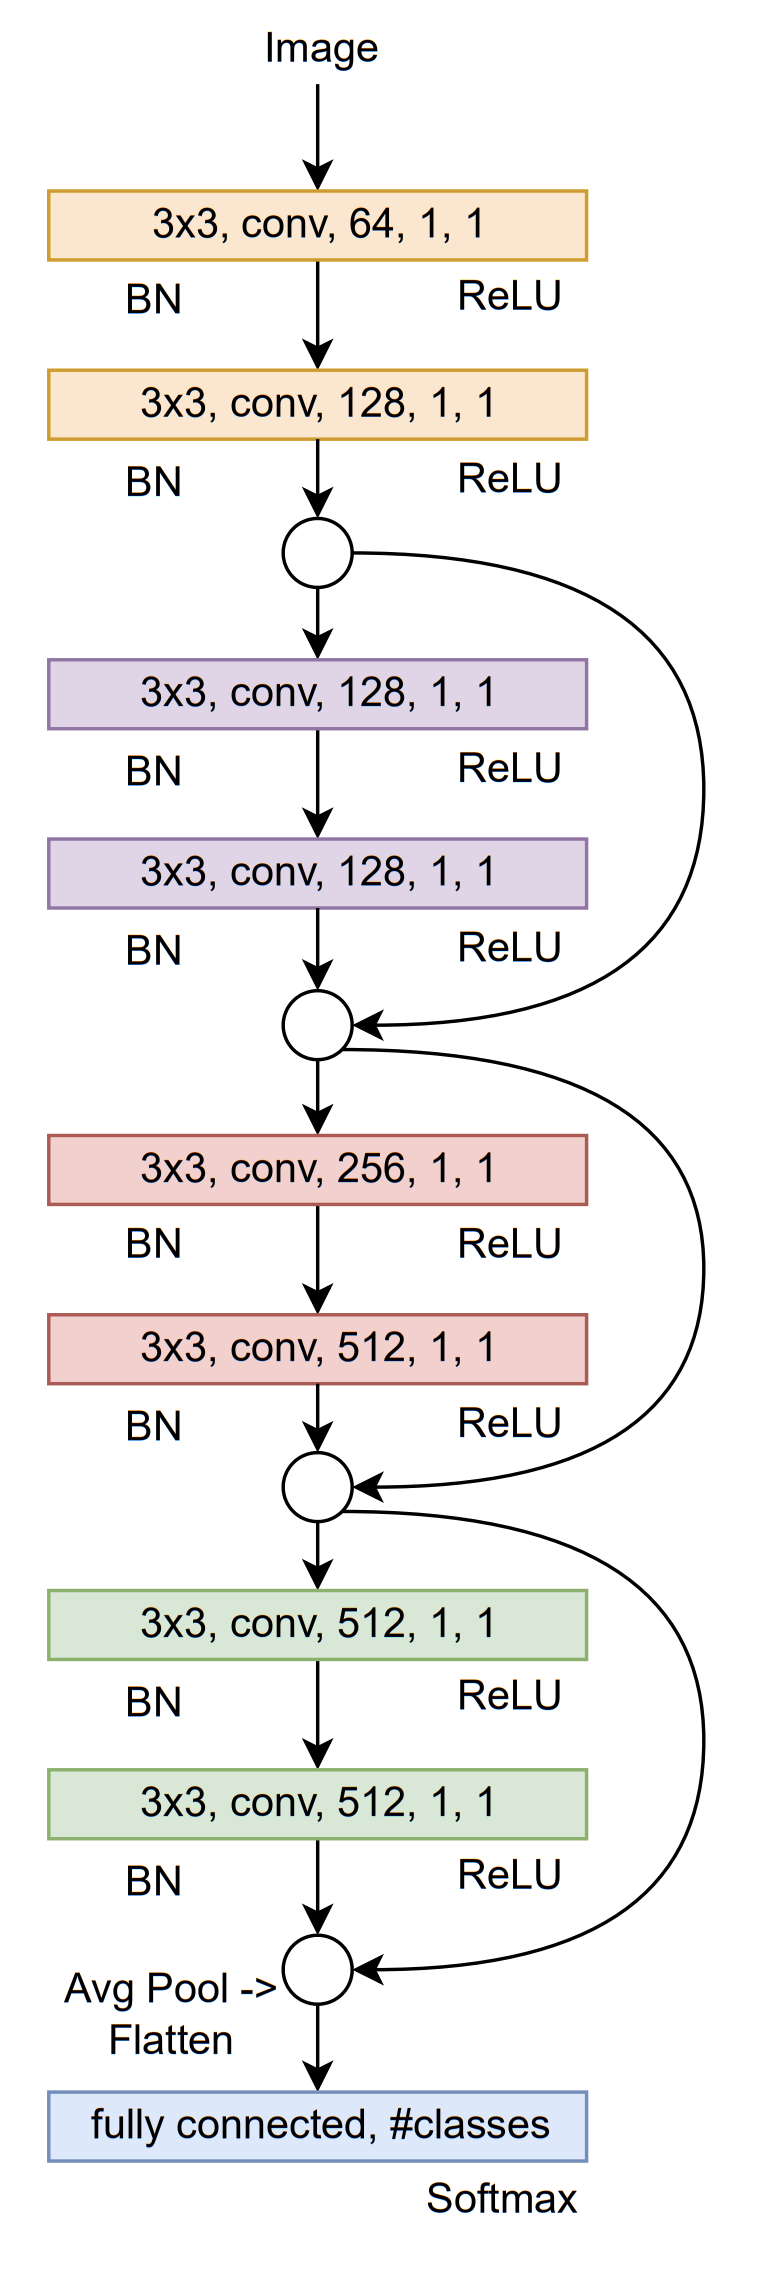
\includegraphics[width=0.25\linewidth]{resnet9.jpg}
\caption{\label{fig:resnet9}The Resnet9 CNN architecture.}
\end{figure}

Common parameters between the models:
\begin{itemize}
\item Number of epochs = 100
\item Maximum Learning Rate = 0.01
\item Gradient Clipping = 0.1
\item Weight Decay = 0.0001
\item Manual random seed (for torch.manual\_seed) = 43
\item Dropout(0.25) for classification layer
\item All the models were run using the T4 GPU runtime on Google colab.
\end{itemize}
The CIFAR-100 dataset: The dataset has not been modified - train-test split is 50000 images for training and 10000 test images. The classification has been conducted on the 100 subclasses.
The dataset has 60000 images (32*32 pixels, 3 channel colour).

\noindent
Note: The temperature for gumbel\_softmax and log\_gumbel\_softmax was $\lambda =  5$, and better metrics can be obtained testing other values of tau. This report does not analyse the nature of the gumbel\_softmax and therefore has only 1 particular example.
\newpage
\subsection{Accuracy}

\begin{table}[h]
\centering
\begin{tabular}{l|r}
Activation function & Accuracy (\%) \\\hline
softmax & 13.37 \\
log\_softmax & 59.16 \\
gumbel\_softmax & 14.84 \\
log\_gumbel\_softmax & 55.87 \\
log\_taylor\_softmax & 49.19 
\end{tabular}
\caption{\label{tab:widgets}Accuracies for the various activation functions.}
\end{table}
\noindent
There is a clear increase in accuracy when we apply the logarithm to the respective standard function.
\newline
\newline
The standard softmaxes can be useful when we want to amplify one class disproportionately over the others, when an ambiguity arises between one or more classes. However, in a classification task with a large number of classes such as the CIFAR-100, the standard softmaxes lose accuracy which is attributed to the fact that the model is unable to distinguish between classes that are similar in appearance but have different labels, due to the exponential amplification of small differences.
\newline
\newline
\noindent
\begin{figure}[h]
\centering
\begin{minipage}{.5\textwidth}
  \centering
  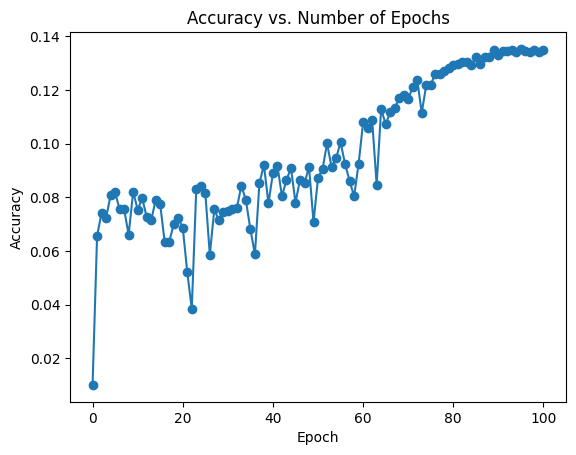
\includegraphics[width=.6\linewidth]{assets/softmax_ae.png}
  \newline
  \noindent
  \captionof{softmax}
  \label{fig:test1}
\end{minipage}%
\begin{minipage}{.5\textwidth}
  \centering
  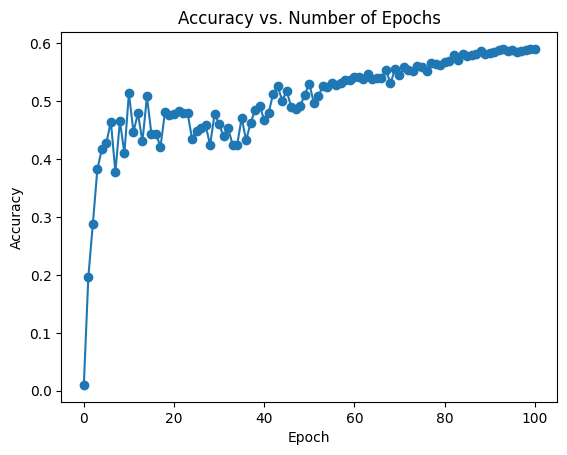
\includegraphics[width=.6\linewidth]{assets/log_softmax_ae.png}
  \newline
  \noindent
  \captionof{log\_softmax}
  \label{fig:test2}
\end{minipage}
\end{figure}
\begin{figure}[h]
\centering
\begin{minipage}{.5\textwidth}
  \centering
  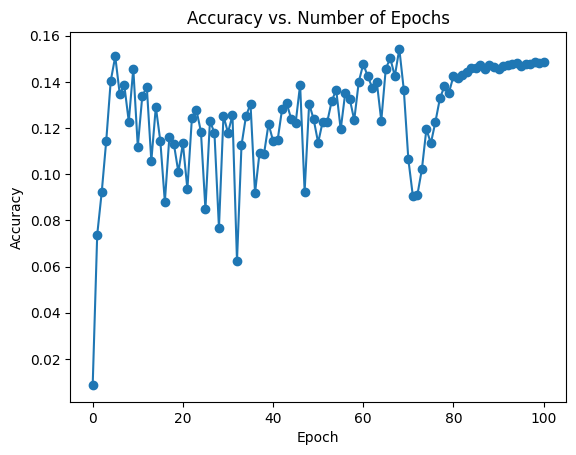
\includegraphics[width=.6\linewidth]{assets/gumbel_softmax_ae.png}
  \newline
  \noindent
  \captionof{gumbel\_softmax}
  \label{fig:test1}
\end{minipage}%
\begin{minipage}{.5\textwidth}
  \centering
  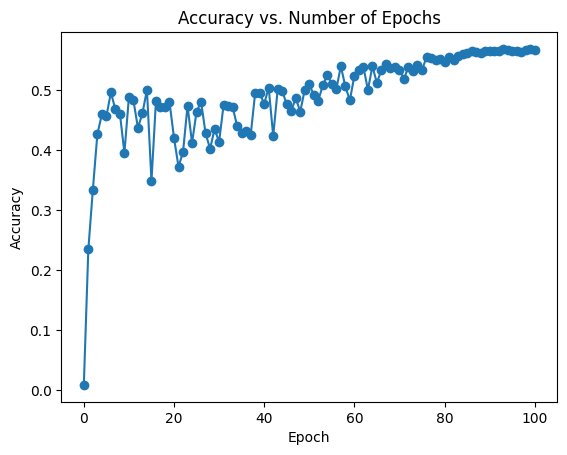
\includegraphics[width=.6\linewidth]{assets/log_gumbel_softmax_ae.png}
  \newline
  \noindent
  \captionof{log\_gumbel\_softmax}
  \label{fig:test2}
\end{minipage}
\end{figure}
\begin{figure}[!h]
\centering
\begin{minipage}{.5\textwidth}
  \centering
  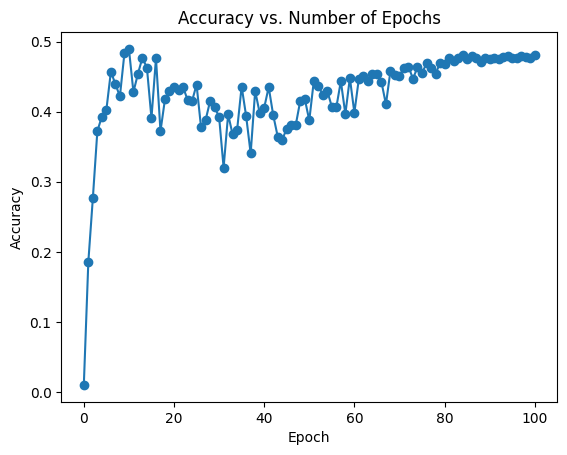
\includegraphics[width=.6\linewidth]{assets/log_taylor_softmax_ae.png}
  \newline
  \noindent
  \captionof{log\_taylor\_softmax}
  \label{fig:test2}
\end{minipage}
\end{figure}
\noindent
\newline
We can observe that non-logarithmic have a very unstable gradient descent pathway as seen by the large fluctuations in accuracy as the epoch number rises. But all models eventually converge by the time the last epoch is reached.

\newpage
\subsection{Precision}

\begin{table}[h]
\centering
\begin{tabular}{l|r}
Activation function & Precision \\\hline
softmax & 0.0280\\
log\_softmax & 0.5891 \\
gumbel\_softmax & 0.0330 \\
log\_gumbel\_softmax & 0.5646\\
log\_taylor\_softmax & 0.5107 
\end{tabular}
\caption{\label{tab:widgets}Precision for the various activation functions.}
\end{table}
\noindent
Here the trend is similar to accuracy where the logarithmic activation outperform their non logarithmic counterparts.

\subsection{Recall}

\begin{table}[h]
\centering

\begin{tabular}{l|r}
Activation function & Recall \\\hline
softmax & 0.1343 \\
log\_softmax & 0.5885 \\
gumbel\_softmax & 0.1496 \\
log\_gumbel\_softmax & 0.5632 \\
log\_taylor\_softmax & 0.4782 
\end{tabular}
\caption{\label{tab:widgets}Recall for the various activation functions.}
\end{table}
\noindent

Here the trend is similar to accuracy where the logarithmic activation outperform their non logarithmic counterparts.


\subsection{F1 Score}

\begin{table}[h]
\centering
\begin{tabular}{l|r}
Activation function & F1 score \\\hline
softmax & 0.0457 \\
log\_softmax & 0.5867 \\
gumbel\_softmax & 0.0533 \\
log\_gumbel\_softmax & 0.5617 \\
log\_taylor\_softmax & 0.4760 
\end{tabular}
\caption{\label{tab:widgets}F1 scores for the various activation functions.}
\end{table}
\noindent
Here the trend is similar to accuracy where the logarithmic activation outperform their non logarithmic counterparts.

\newpage
\subsection{Confusion Matrices}
\begin{figure}[h]
\centering
\begin{minipage}{.5\textwidth}
  \centering
  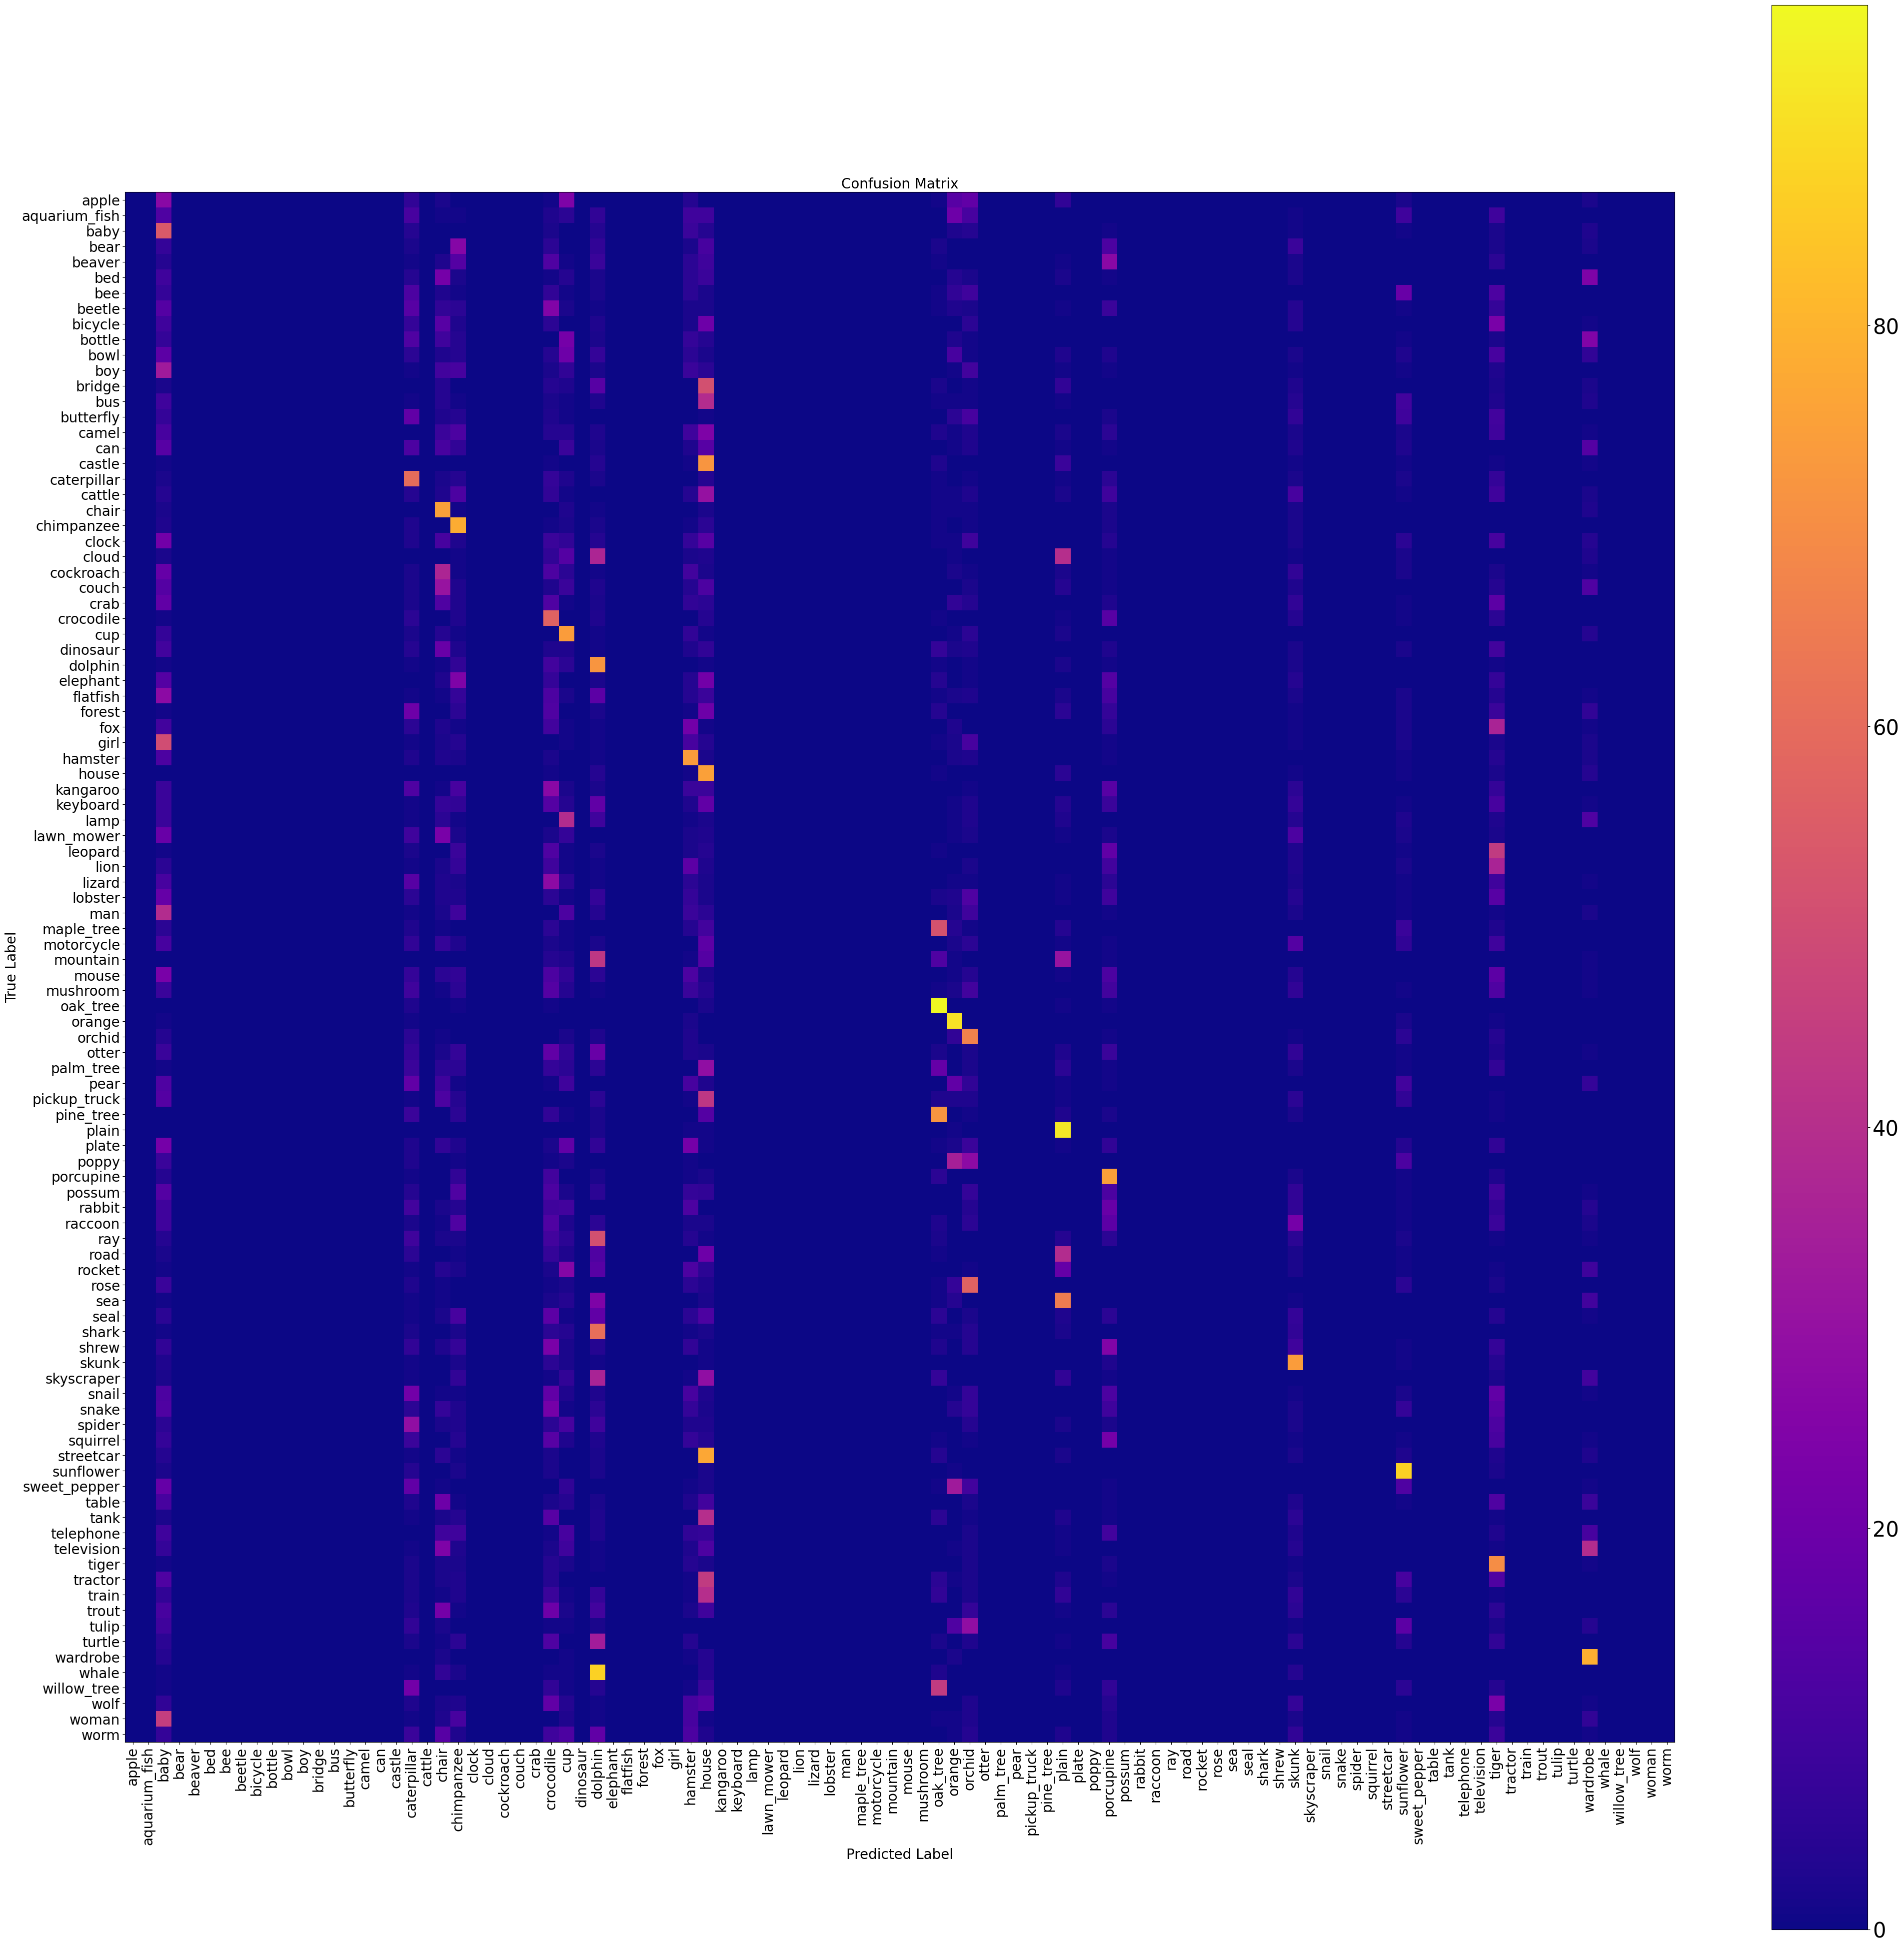
\includegraphics[width=.6\linewidth]{assets/softmax_cm.png}
  \newline
  \noindent
  \captionof{softmax}
  \label{fig:test1}
\end{minipage}%
\begin{minipage}{.5\textwidth}
  \centering
  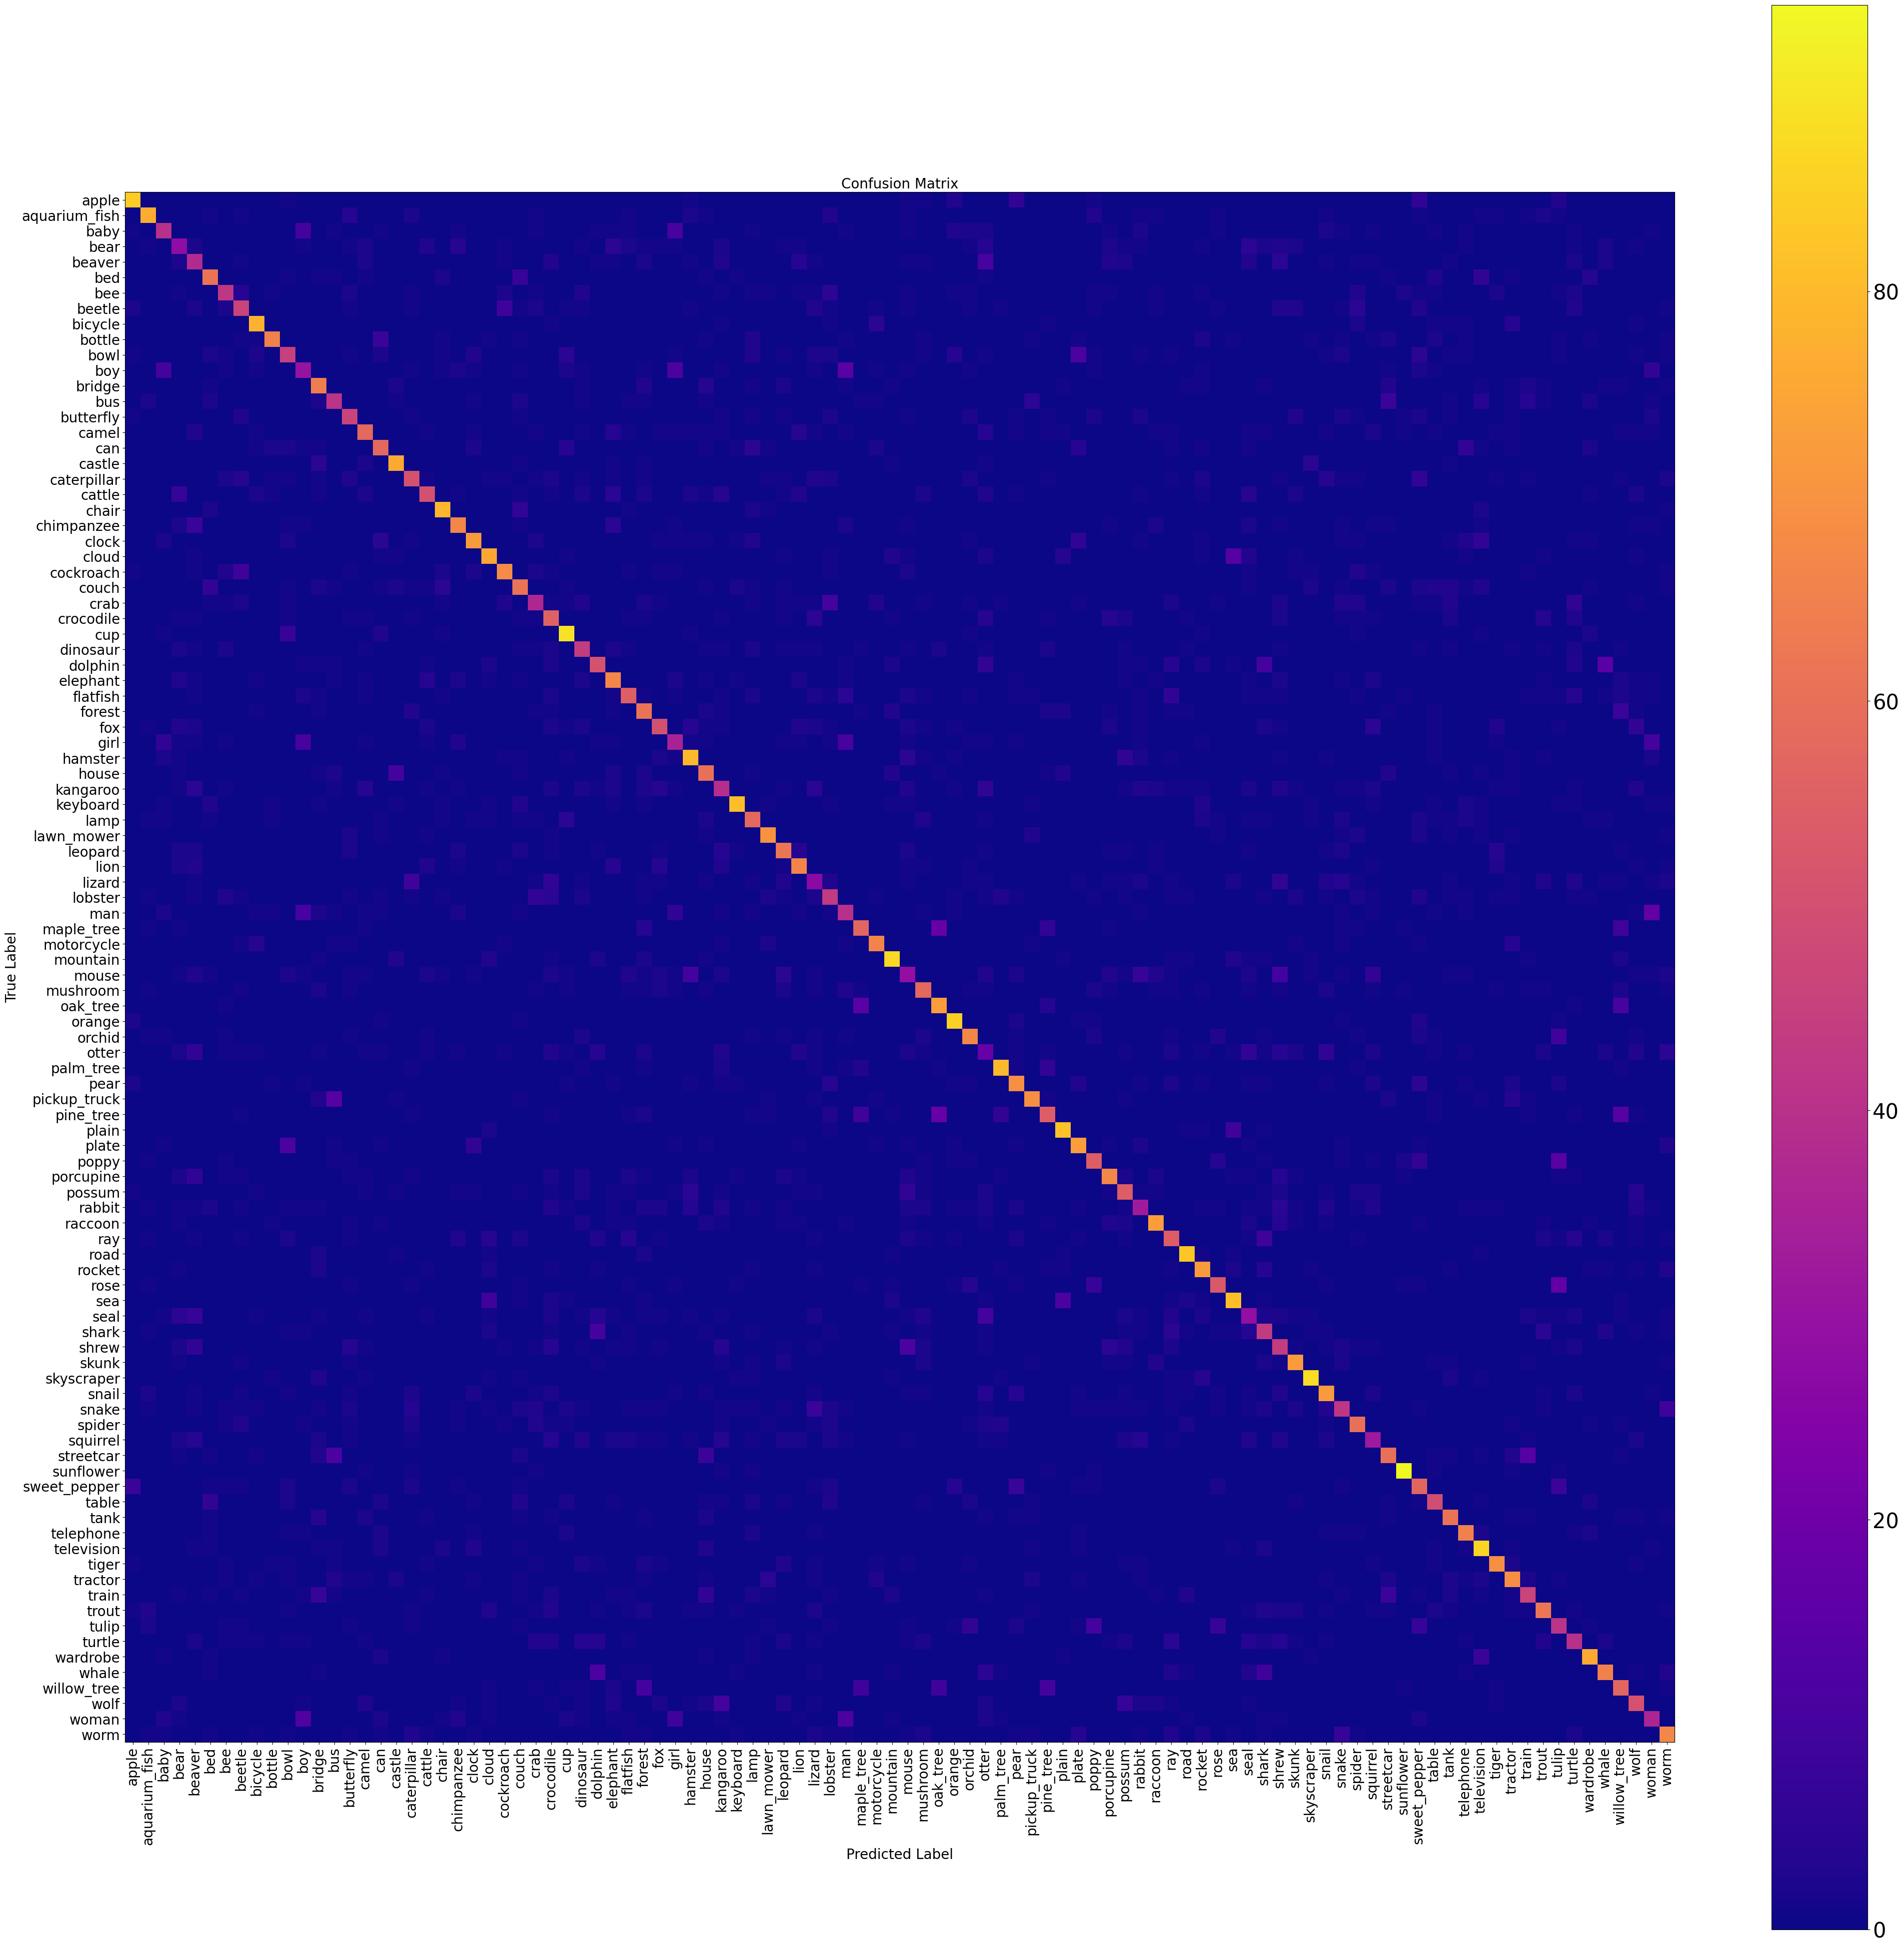
\includegraphics[width=.6\linewidth]{assets/log_softmax_cm.png}
  \newline
  \noindent
  \captionof{log\_softmax}
  \label{fig:test2}
\end{minipage}
\end{figure}

\begin{figure}[h]
\centering
\begin{minipage}{.5\textwidth}
  \centering
  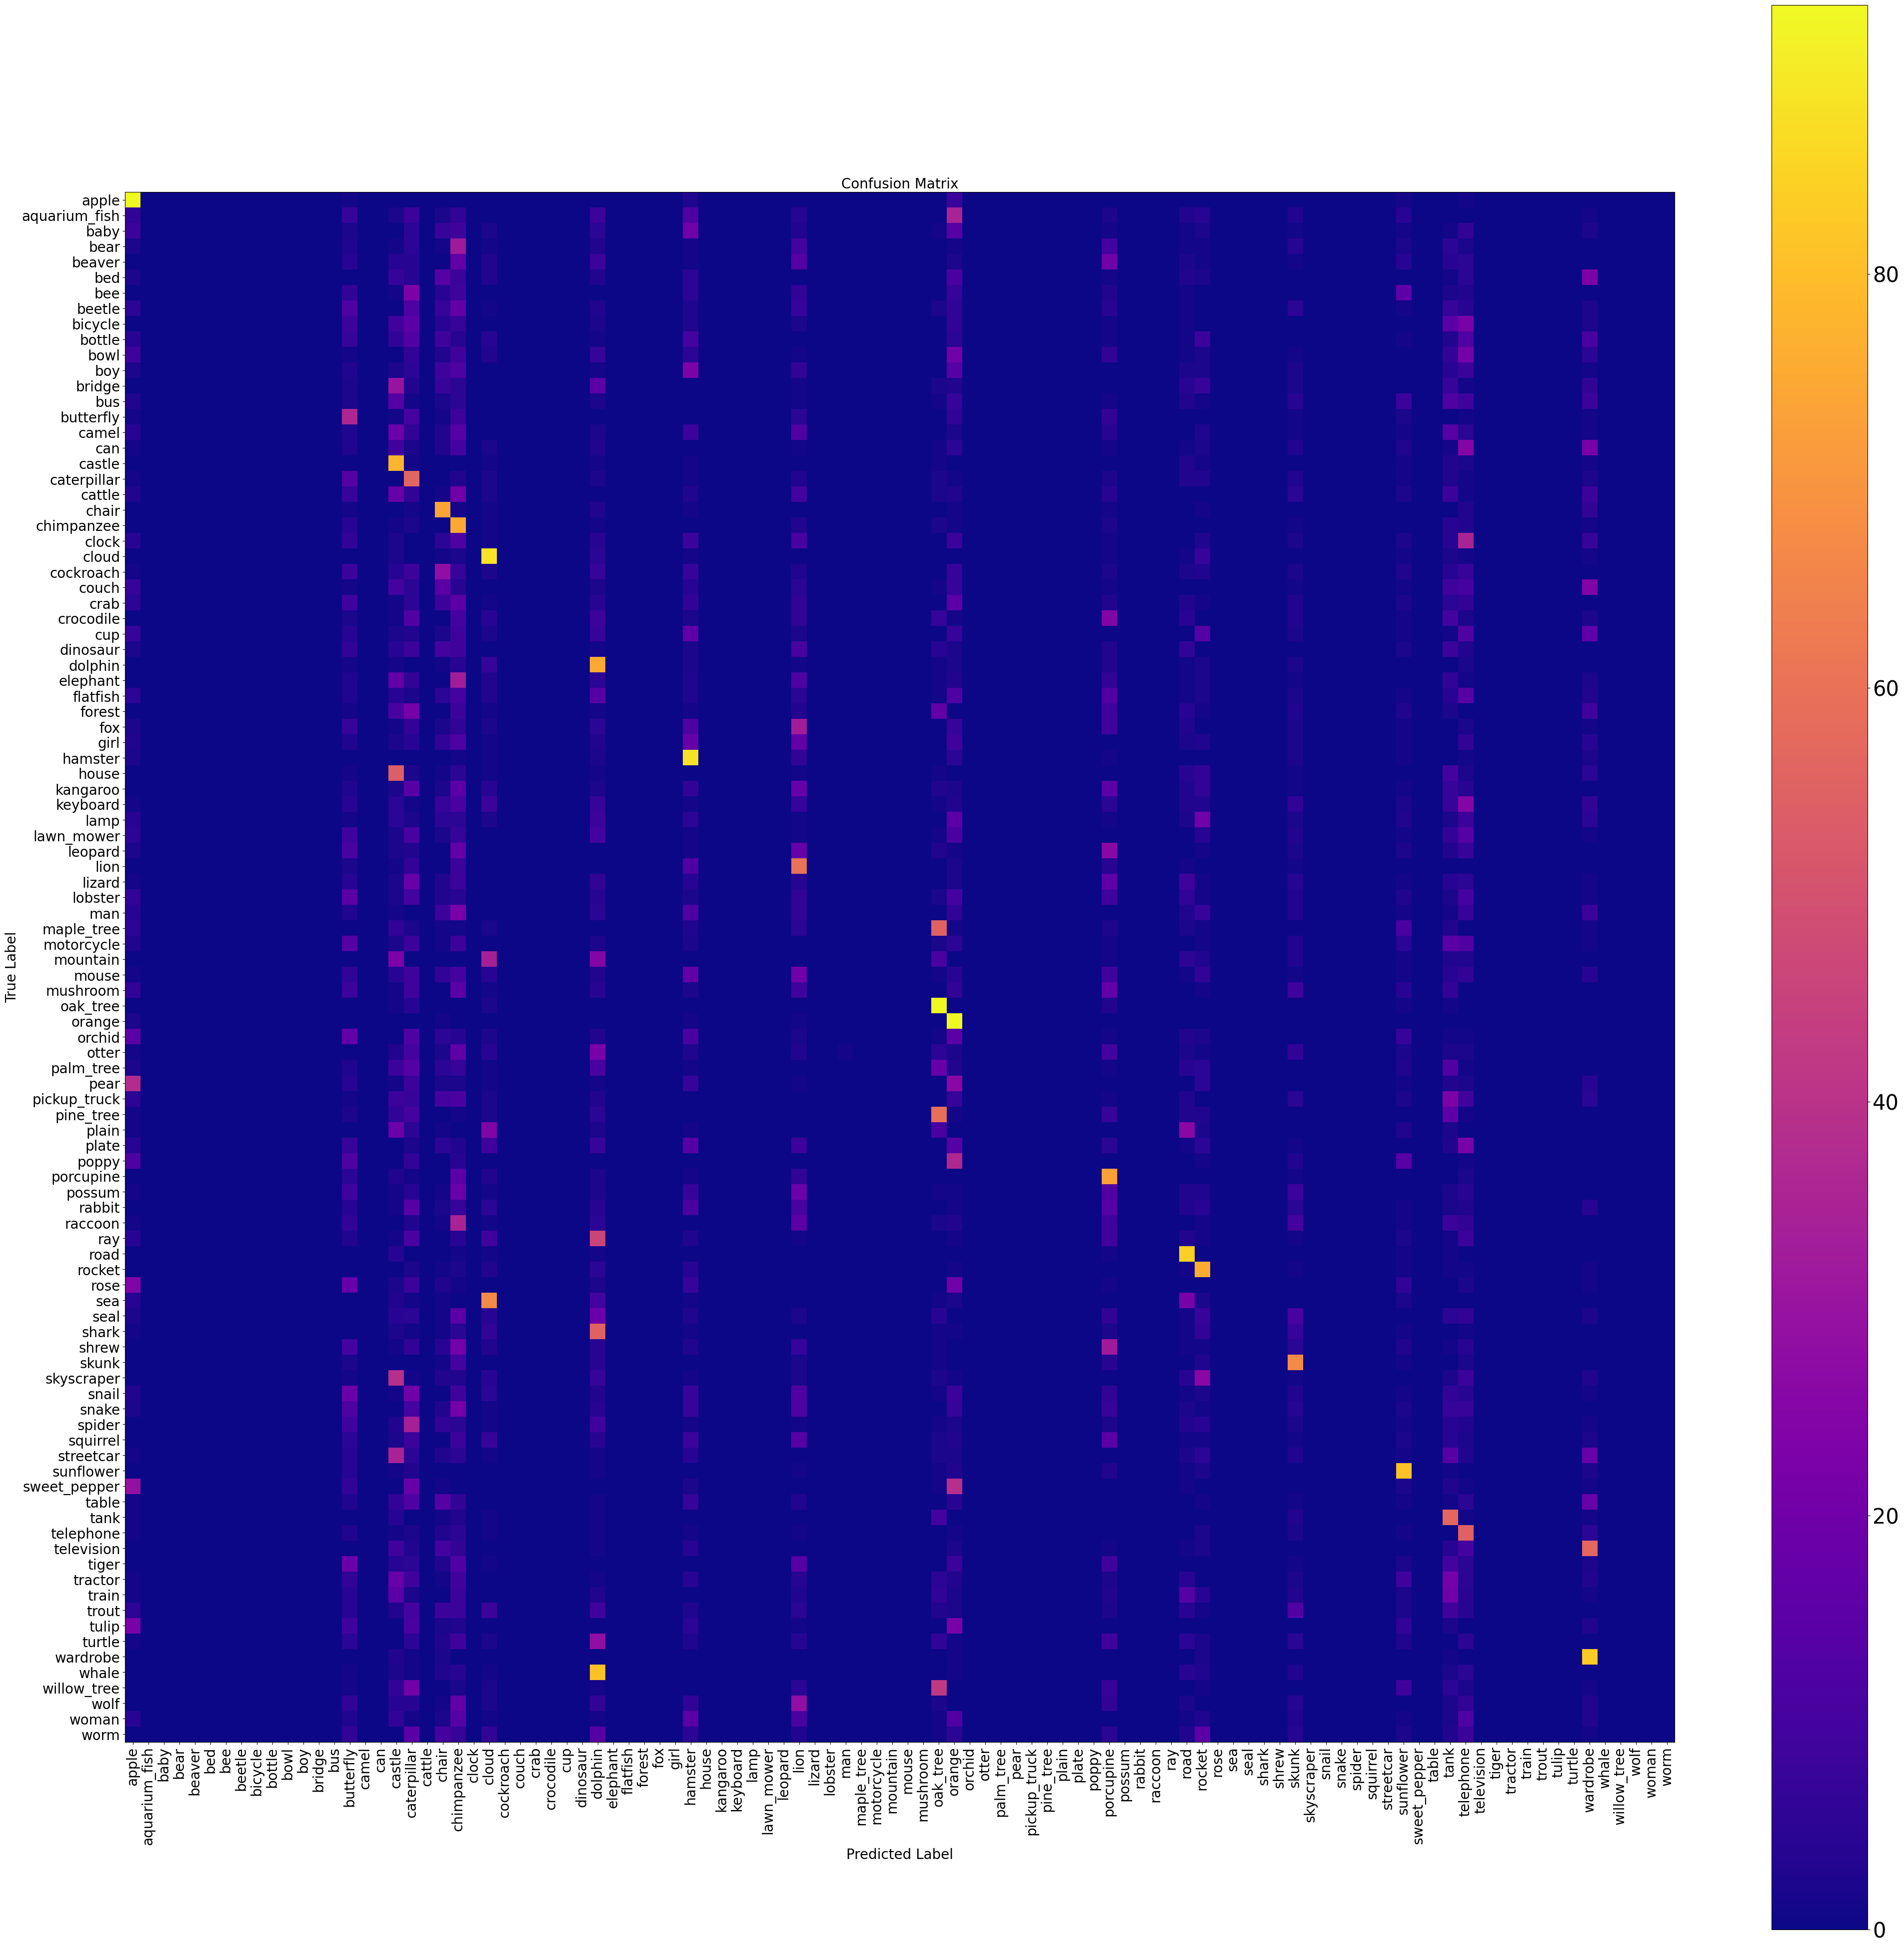
\includegraphics[width=.6\linewidth]{assets/gumbel_softmax_cm.png}
  \newline
  \noindent
  \captionof{gumbel\_softmax}
  \label{fig:test1}
\end{minipage}%
\begin{minipage}{.5\textwidth}
  \centering
  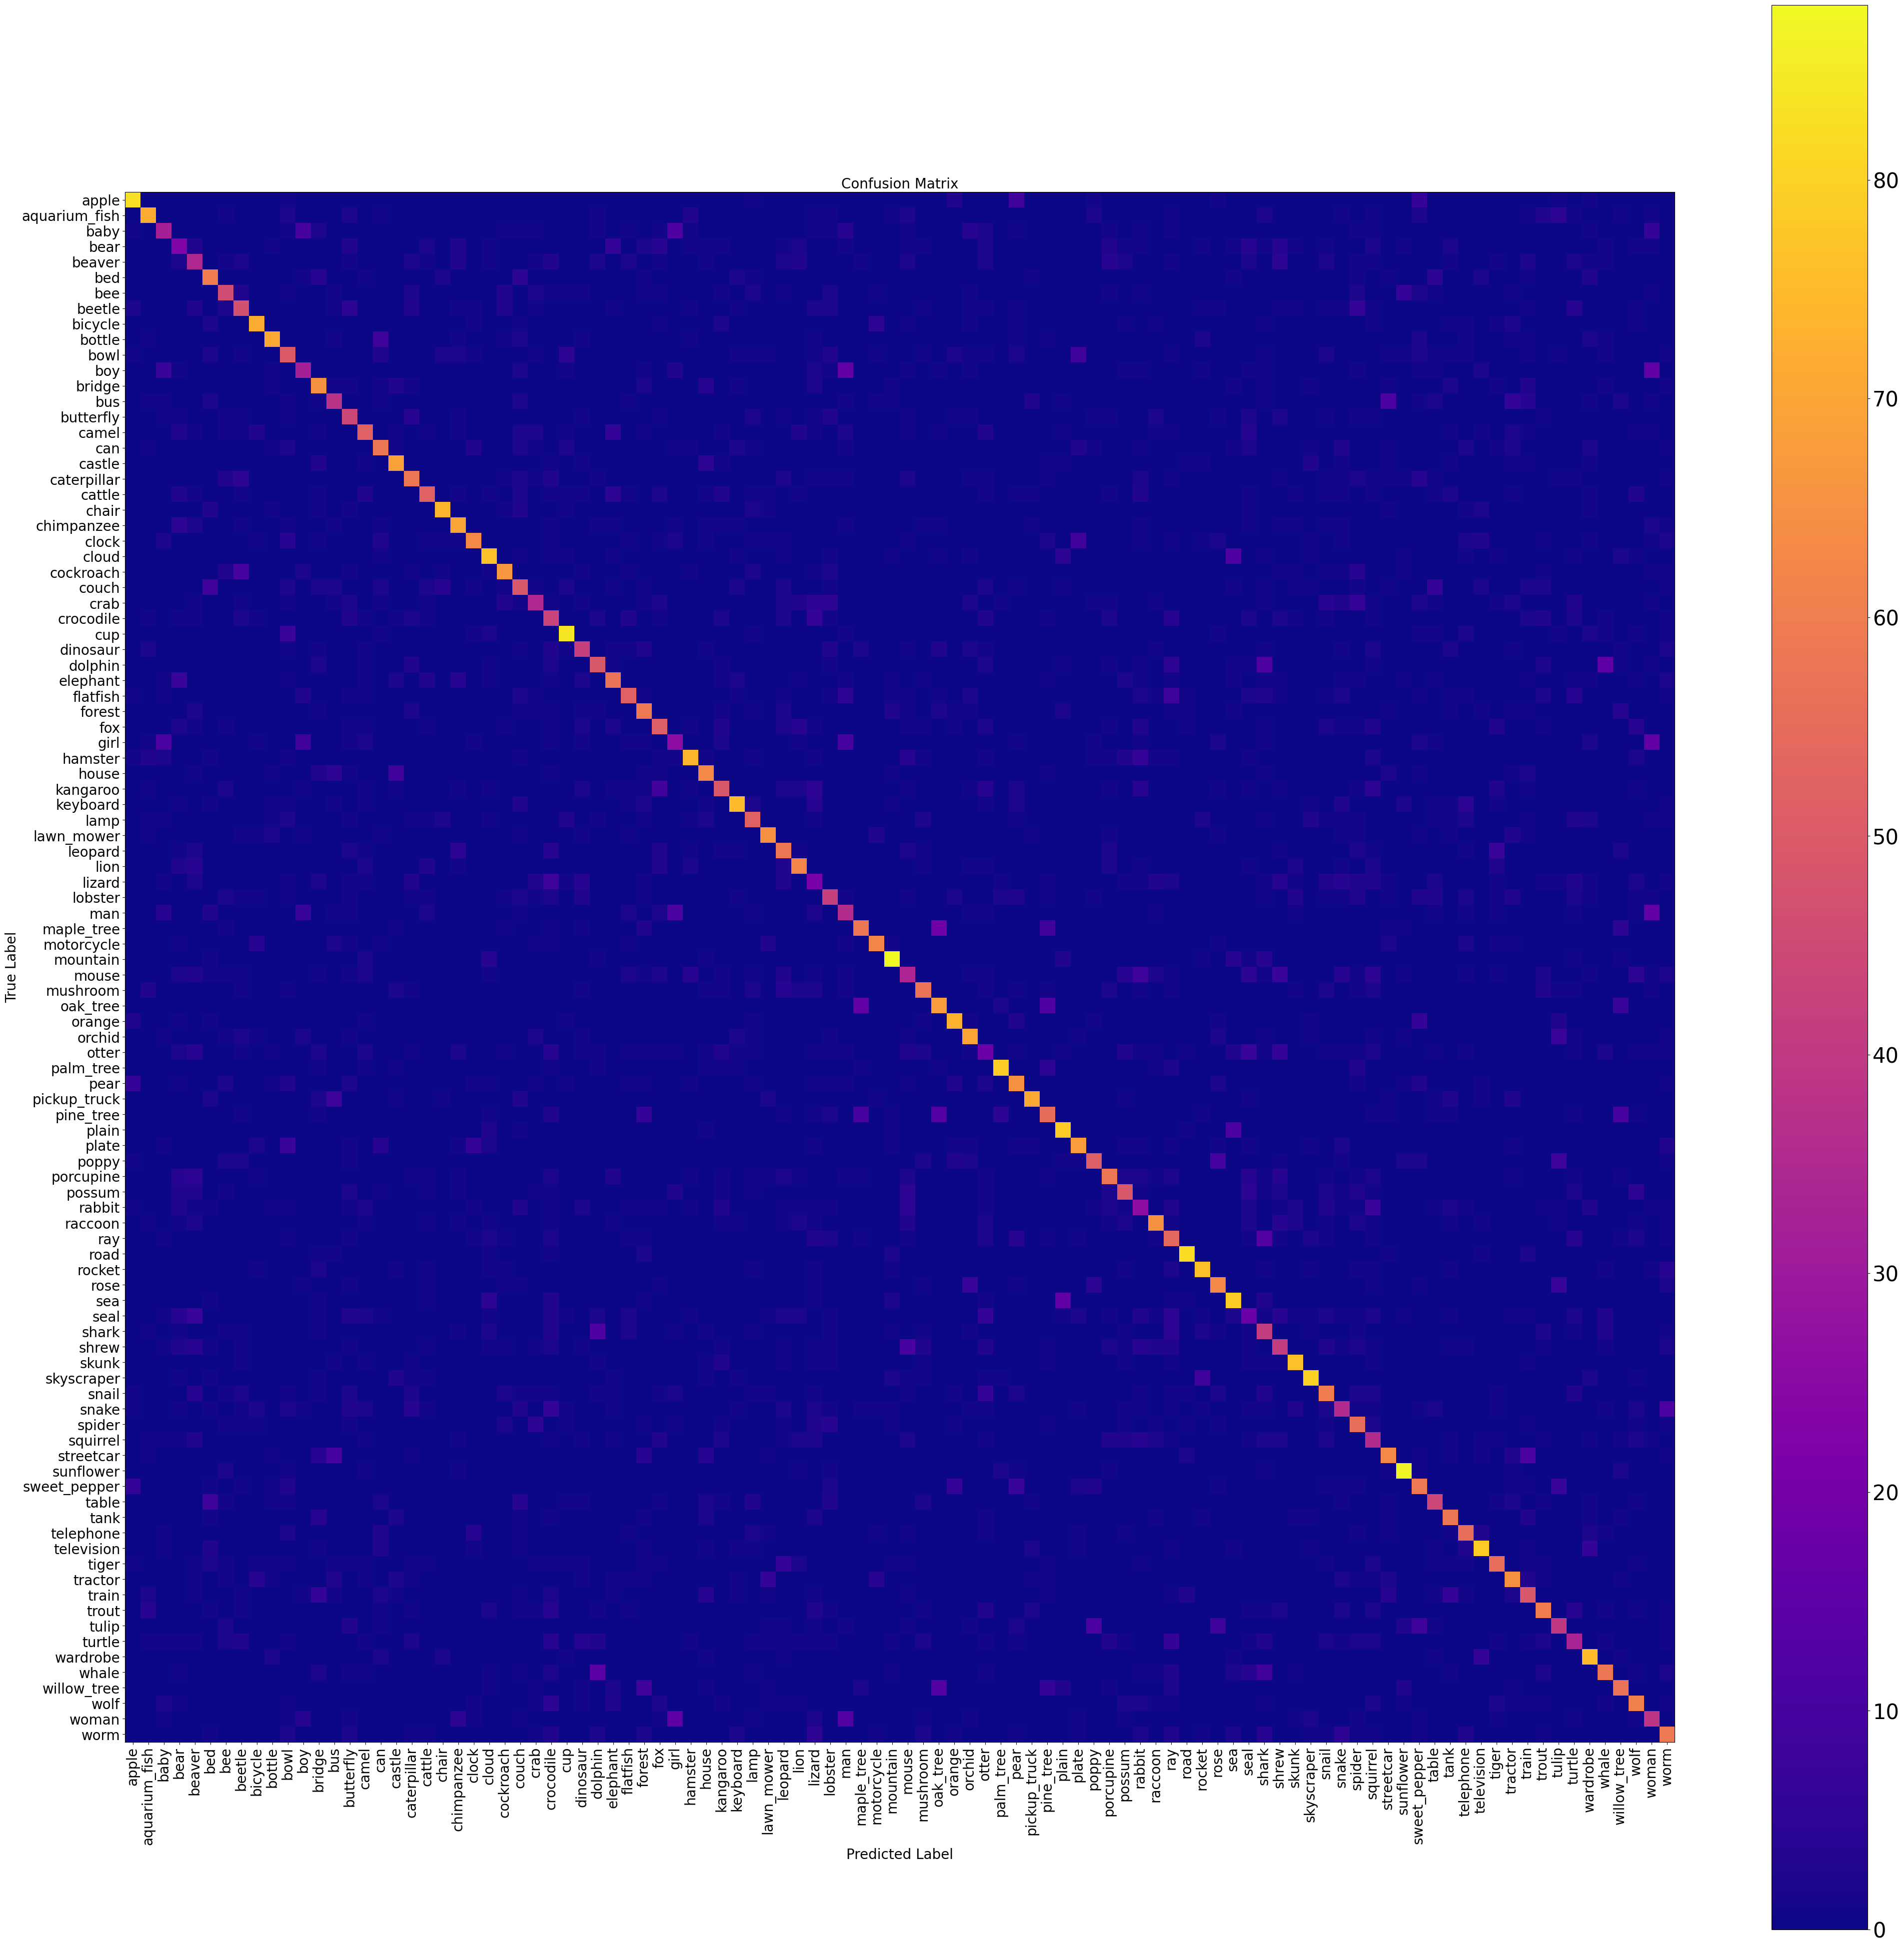
\includegraphics[width=.6\linewidth]{assets/log_gumbel_softmax_cm.png}
  \newline
  \noindent
  \captionof{log\_gumbel\_softmax}
  \label{fig:test2}
\end{minipage}
\end{figure}
\begin{figure}[h]
\centering
\begin{minipage}{.5\textwidth}
  \centering
  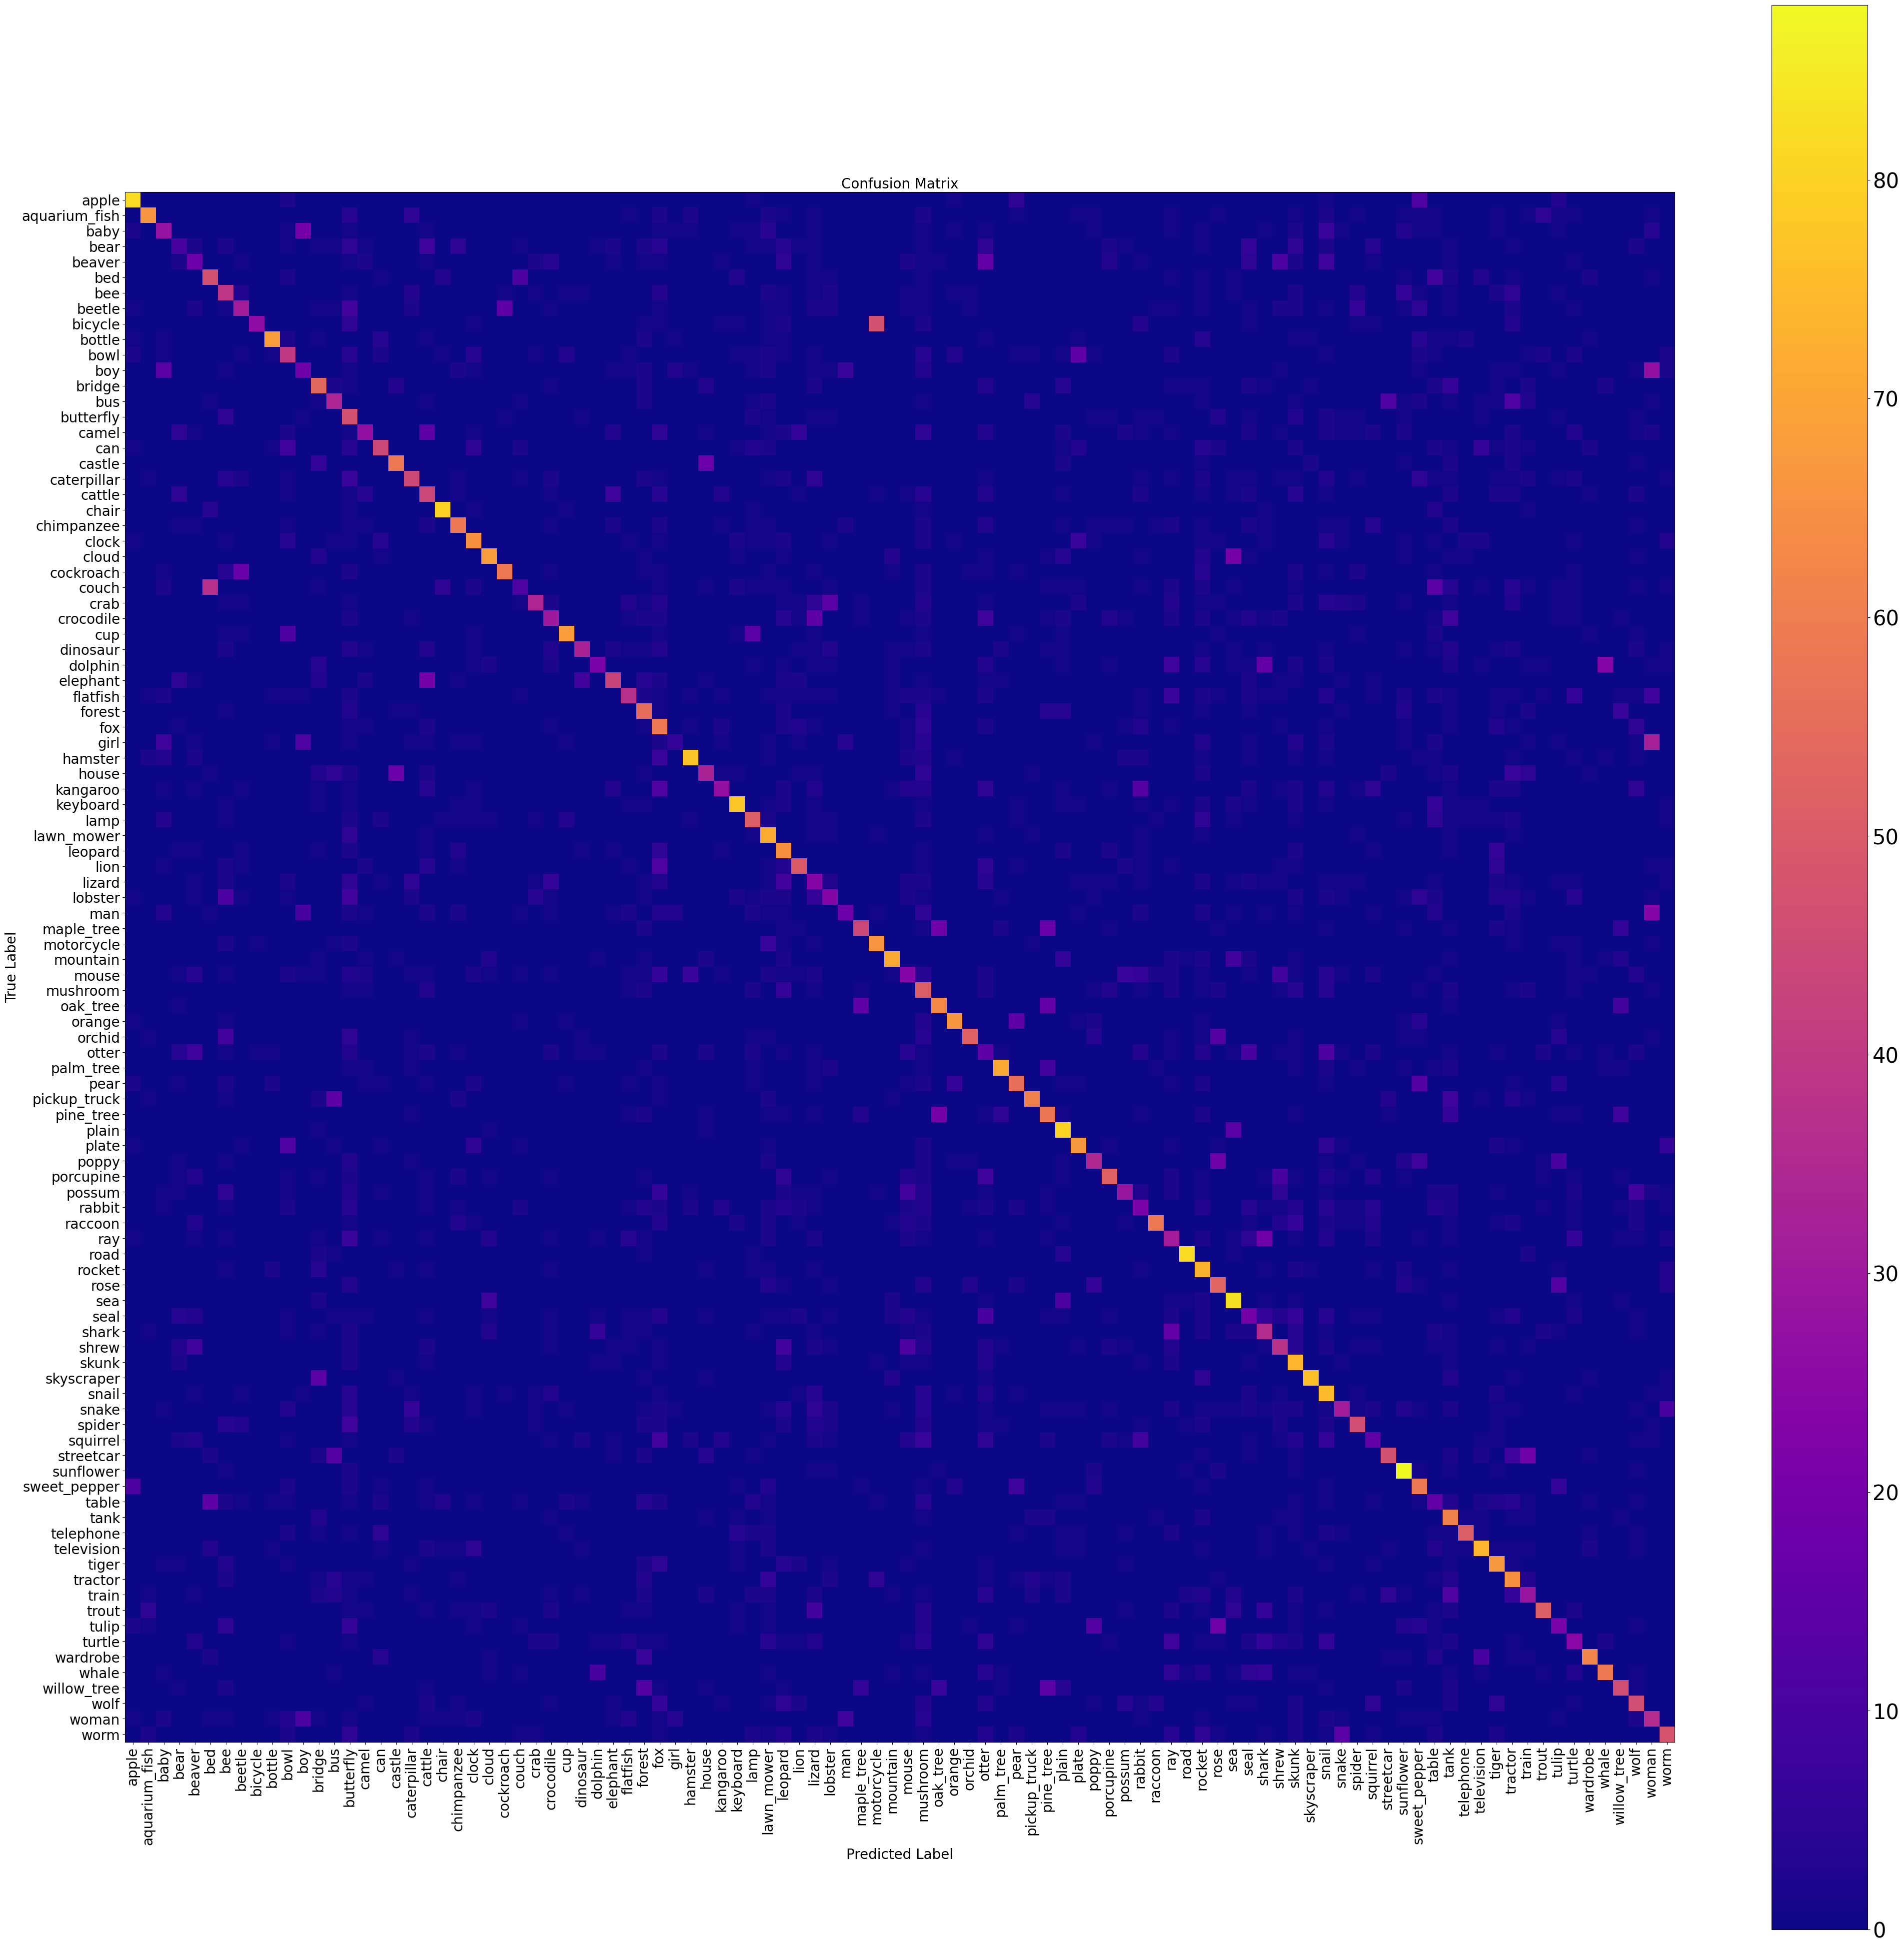
\includegraphics[width=.6\linewidth]{assets/log_taylor_softmax_cm.png}
  \newline
  \noindent
  \captionof{log\_taylor\_softmax}
  \label{fig:test2}
\end{minipage}
\end{figure}

\noindent
We observe that the logarithmic activations produce classifiers with much more well defined confusion matrices.
\newpage
\subsection{Epoch time}
Epoch time has been calculated as:
\[ \text{epoch time} = \frac{\text{wall time after 100 epochs}}{100}\]
\newline

\begin{table}[h]
\centering
\begin{tabular}{l|r}
Activation function & Epoch time (seconds) \\\hline
softmax & 19.95\\
log\_softmax & 20.33 \\
gumbel\_softmax & 19.64 \\
log\_gumbel\_softmax & 21.07\\
log\_taylor\_softmax & 20.59 
\end{tabular}
\caption{\label{tab:widgets}Epoch time for the various activation functions.}
\end{table}
\noindent
We observe that there is a minor time penalty associated with taking the logarithm, however we see log\_softmax is the fastest logarithmic softmax, and gumbel\_softmax is faster than the standard softmax.
\newline
\noindent
However the models having a logarithmic softmax have finished training around ~25 epochs earlier than the non-logarithmic softmaxes, so they train around ~20\% faster since they need lesser epochs to reach their minimal loss.

\newpage
\subsection{Loss v/s epochs}
\begin{figure}[h]
\centering
\begin{minipage}{.5\textwidth}
  \centering
  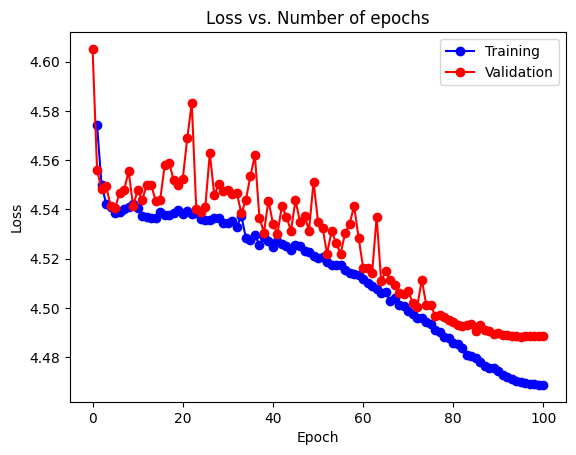
\includegraphics[width=.6\linewidth]{assets/softmax_le.png}
  \newline
  \noindent
  \captionof{softmax}
  \label{fig:test1}
\end{minipage}%
\begin{minipage}{.5\textwidth}
  \centering
  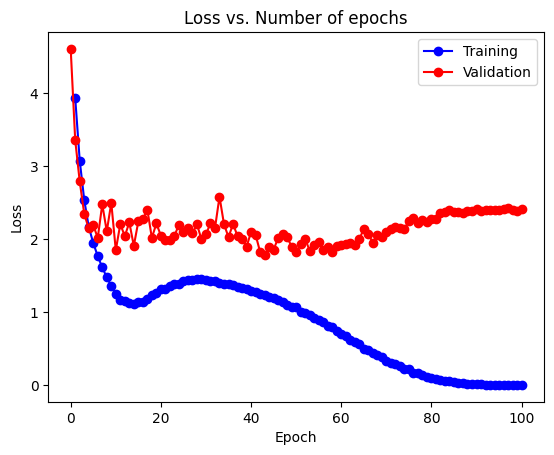
\includegraphics[width=.6\linewidth]{assets/log_softmax_le.png}
  \newline
  \noindent
  \captionof{log\_softmax}
  \label{fig:test2}
\end{minipage}
\end{figure}

\begin{figure}[h]
\centering
\begin{minipage}{.5\textwidth}
  \centering
  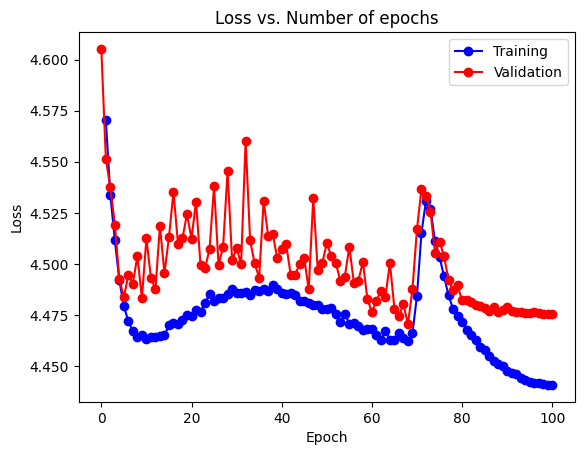
\includegraphics[width=.6\linewidth]{assets/gumbel_softmax_le.png}
  \newline
  \noindent
  \captionof{gumbel\_softmax}
  \label{fig:test1}
\end{minipage}%
\begin{minipage}{.5\textwidth}
  \centering
  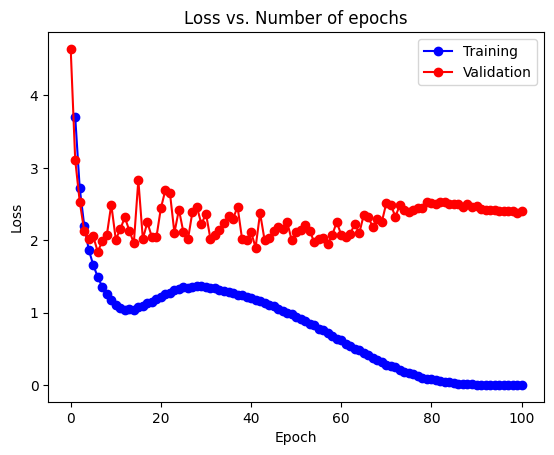
\includegraphics[width=.6\linewidth]{assets/log_gumbel_softmax_le.png}
  \newline
  \noindent
  \captionof{log\_gumbel\_softmax}
  \label{fig:test2}
\end{minipage}
\end{figure}
\begin{figure}[h]
\centering
\begin{minipage}{.5\textwidth}
  \centering
  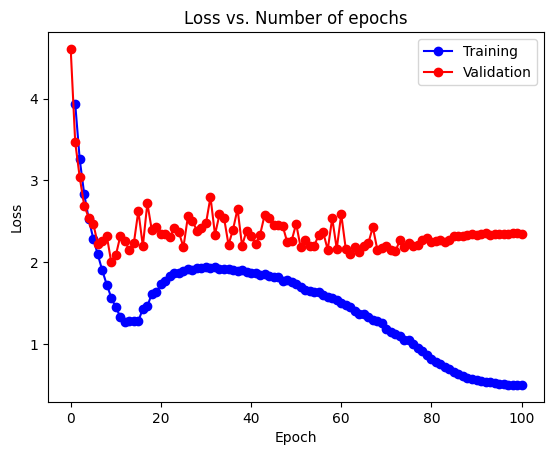
\includegraphics[width=.6\linewidth]{assets/log_taylor_softmax_le.png}
  \newline
  \noindent
  \captionof{log\_taylor\_softmax}
  \label{fig:test2}
\end{minipage}
\end{figure}
\noindent
We can see that the training and validation losses are more closely associated with each other and diverge much slowly in the non-logarithmic softmaxes.
The logarithmic softmaxes reach their divergence point quicker and the loss stabilizes around the $75^{th}$ epoch, meaning the models have finished training earlier.
\newline
\newline
\noindent
In addition to finishing training in lesser epochs, the logarithmic softmaxes also minimize the loss more than their non-logarithmic counterparts.
\newpage
\section{Conclusions}
To conclude, I have found that taking the logarithm of the standard softmax variations outperform the non-logarithmic versions in every metric analysed here.
However these results may not hold true for datasets with lower number of classes such as the MINST dataset where the softmax function benefits the model by reducing uncertainty.
gumbel\_softmax is more performant than the standard softmax, and its efficacy can be improved by optimising the $\lambda$ or temperature parameter.
The log-Softmax is the most performant of the logarithmic softmaxes, however the performance of the log\_taylor\_softmax can be adjusted by adjusting the order of the Taylor polynomial to which we calculate, which requires further examination.


\section{Sources/References}
Kunal Banerjee et al, "Exploring Alternatives to Softmax Function", 2020,  https://arxiv.org/pdf/2011.11538.pdf
\newline\newline
Figure 1 from: Chandramouli Rajagopalan et al, "Deep learning in a bilateral brain with hemispheric specialization", 2023, https://arxiv.org/pdf/2209.06862.pdf
\newline\newline
Youngkyu Hong et al, Disentangling Label Distribution for Long-tailed Visual Recognition, 2021, https://arxiv.org/pdf/2012.00321v2.pdf
\newline\newline
Introduction to Softmax for Neural Network, https://www.analyticsvidhya.com/blog/2021/04/introduction-to-softmax-for-neural-network/
\newline\newline
Softmax: Multiclass Neural Networks, https://www.turing.com/kb/softmax-multiclass-neural-networks
\newline\newline
Train your image classifier model with PyTorch, https://learn.microsoft.com/en-us/windows/ai/windows-ml/tutorials/pytorch-train-model
\newline\newline
Image Classification in a Nutshell: 5 Different Modelling Approaches in PyTorch with CIFAR100, https://medium.com/@alitbk/image-classification-in-a-nutshell-5-different-modelling-approaches-in-pytorch-with-cifar100-8f690866b373
\newline\newline
Softmax and Uncertainty, https://towardsdatascience.com/softmax-and-uncertainty-c8450ea7e064
\newline\newline
https://github.com/Harshvardhan-Mestha/SAiDL\_Assignment



\end{document}